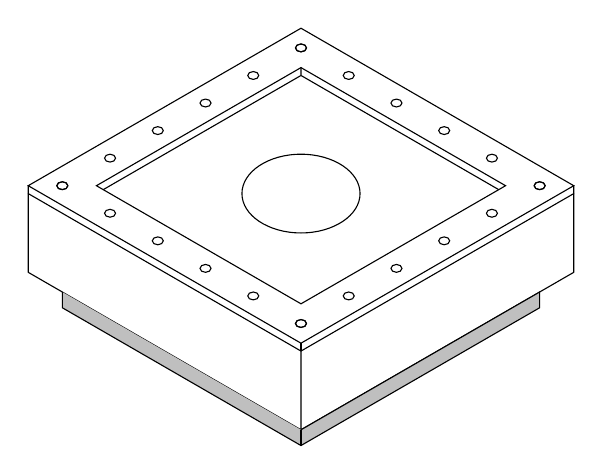
\begin{tikzpicture}
%top
\draw (0,0) -- ++ (30:4) -- ++ (0,0.1)
(0,0) -- ++ (150:4) -- ++ (0,0.1);
%circle
\draw (0,2) circle [x radius=0.75, y radius=0.5];

%edges
\draw (0,0) -- ++ (0,-1) coordinate (middle)
(0,0) ++ (30:4) -- ++ (0,-1) coordinate (left)
(0,0) ++ (150:4) -- ++ (0,-1) coordinate (right)
(left) -- (middle) -- (right);

%sample
\draw [fill = lightgray]
(0,-1) -- ++ (30:3.5) -- ++ (0,-0.2) -- ++ (210:3.5) -- ++ (150:3.5) -- ++ (0,.2);
\draw (0,-1) -- (0,-1.2);

%steel frame
\draw (0,0) -- ++ (0,0.1); 
\draw (0,0.1) -- ++ (30:4) -- ++  (150:4) -- ++ (210:4) -- cycle;
\draw (0,0.6) -- ++ (30:3) -- ++  (150:3) coordinate (up) -- ++ (210:3) -- cycle;
\draw (up) -- ++ (0,-0.1)
(up) ++ (0,-0.1) -- ++ (210:2.9)
(up) ++ (0,-0.1) -- ++ (330:2.9);
%bolts
\foreach \x in {0, 0.7,...,3.5}
{
\draw (0,0) ++ (0,0.35) ++ (30:\x) circle [x radius=0.07, y radius=0.05];
\draw (0,0) ++ (0,0.35) ++ (150:\x) circle [x radius=0.07, y radius=0.05];
\draw (0,0) ++ (0,0.35) ++ (150:3.5) ++ (30:\x) circle [x radius=0.07, y radius=0.05];
\draw (0,0) ++ (0,0.35) ++ (30:3.5) ++ (150:\x) circle [x radius=0.07, y radius=0.05];
}
%hooks

\end{tikzpicture}